\documentclass[11pt]{article}

% ---------- Packages ----------
\usepackage[margin=1in]{geometry}
\usepackage{times}
\usepackage[utf8]{inputenc}
\usepackage[T1]{fontenc}
\usepackage{graphicx}
\usepackage{booktabs}
\usepackage{caption}
\usepackage{subcaption}
\usepackage{amsmath}
\usepackage[table]{xcolor}
\usepackage{hyperref}
\usepackage{xurl}
\usepackage[round]{natbib}
\usepackage{setspace}
\usepackage{titlesec}
\usepackage{enumitem}

% ---------- Consistent color palette (used across all figures & tables) ----------
% Primary: deep indigo (low risk) -> warm coral (high risk); neutral gray for reference lines
\definecolor{paletteLow}{HTML}{3B4F8C}
\definecolor{paletteHigh}{HTML}{E0673E}
\definecolor{paletteAccent}{HTML}{2E8B7E}
\definecolor{paletteGray}{HTML}{6B6B6B}
\definecolor{tableheader}{HTML}{EFEFEF}

\hypersetup{
  colorlinks=true,
  linkcolor=paletteLow,
  citecolor=paletteLow,
  urlcolor=paletteLow
}

\titleformat{\section}{\normalfont\Large\bfseries}{\thesection}{1em}{}
\titleformat{\subsection}{\normalfont\large\bfseries}{\thesubsection}{1em}{}
\titleformat{\subsubsection}{\normalfont\normalsize\bfseries\itshape}{\thesubsubsection}{1em}{}

\setlength{\parindent}{1.5em}
\onehalfspacing

\title{\textbf{How Proximity of Metro Stops Relates to Gentrification of Local Neighborhoods}}
\author{
  Jon Darius \and Mercy Eme \and Judith Mendoz \and Layla Rainosek \and Daniel Rocha \\
  \small MAS405, Spring 2026 \\
  \small University of California, Los Angeles
}
\date{\today}

\begin{document}

\maketitle

\begin{abstract}
\noindent
The planned D Line (Purple Line) extension to Westwood/UCLA, scheduled to open ahead of the 2028 Los Angeles Olympic Games, raises the question of whether new transit access will accelerate gentrification in the surrounding Olympic Corridor. We construct a Composite Gentrification Risk Score (CGRS) -- a five-component, z-scored index combining rent premium, rent burden, spatial rent appreciation, price-per-square-foot premium, and education change -- for 15,889 Los Angeles rental listings located within five miles of an existing Metro rail station. Using a one-sided Mann-Whitney $U$ test, we find that listings inside the 0.5-mile transit-oriented development (TOD) buffer have significantly higher CGRS (median $=0.125$) than listings outside it (median $=-0.112$, $U = 25{,}290{,}586$, $p<0.001$), consistent with the TOD-gentrification hypothesis. We then train Ordinary Least Squares, Ridge, Random Forest, and XGBoost models -- restricted to listings nearest the A and E Lines, which we argue are the corridors most comparable to the D Line Westwood extension -- and evaluate them with 5-fold cross-validation. The XGBoost model achieves the lowest cross-validated error (CV-RMSE $= 0.173 \pm 0.005$, CV-$R^2 = 0.885$) and is used to run a counterfactual forecast: for listings within five kilometers of the four planned Olympic-corridor stations, we compare predicted CGRS under current conditions against predicted CGRS as if the stations were already open. The estimated median uplift is small and slightly negative ($\Delta \text{median} \approx -0.013$), indicating that the immediate Westwood/UCLA segment is unlikely to see a meaningful, transit-attributable increase in gentrification risk beyond its already-high baseline. We interpret this as a ``ceiling effect'': the corridor has largely already gentrified, leaving little additional room for transit access alone to move the index. We argue, however, that this does not mean the D Line extension is gentrification-neutral -- rather, that displacement pressure is more likely to surface in adjacent, comparatively affordable communities such as Koreatown, Palms, and Mar Vista, which stand to gain regional accessibility without the same price ceiling. We discuss the implications of these findings for transit-oriented housing policy and outline the limitations of a cross-sectional, predictive (rather than causal) design.
\end{abstract}

\vspace{1em}

% =====================================================================
\section{Introduction}
% =====================================================================

As the Los Angeles (LA) public transit system pushes to grow and accommodate a wider span of neighborhoods within its metro rail line, the concern of transit accessibility should not stop at travel time alone. LA has experienced a mass exodus in recent years due, in large part, to the steep cost of living and housing prices throughout the county \citep{flemming2026thousands}; however, sustained high demand from high-income individuals moving into local areas has continued to drive rent prices up instead of allowing them to stabilize \citep{mcmillen2020fair, walters2024housing}. Shifting the landscape in LA to price out lower-income individuals would be a devastating loss to the culture and vibrancy of the city, and dedicating attention to the possibility of gentrification in certain areas is a necessary first step in combating this issue.

Though population growth has steadily slowed in LA over the past several years \citep{ferrara2026population, worldpopulationreview2026la}, demand for living in LA is still high due to its attractiveness as a location and vibrant culture. Anecdotally, one of the largest deterrents to living in LA is its notorious traffic; however, with the push to remove this obstacle by improving the public transit system, demand for housing may drive out long-time residents who are unable to keep up with rental prices. Proximity to a public transit system is often listed as an amenity on rental websites \citep{apta2019locations}, which can increase the perception of fair market price for a rental unit. However, a surge in rental prices can instigate a wave of gentrification in low-income neighborhoods and disproportionately affect Black and Latino communities throughout the city \citep{rucksahidiana2022theorizing}. Inadvertent negative outcomes resulting from public services have been theoretically linked \citep{debrezion2007impact}, though research across different cities has revealed case-specific outcomes that connect public transit and gentrification.

Previous research has yielded mixed results on the affordability of LA housing as it relates to access to public transportation, finding that single-family homes were marginally less expensive when close to nearby Metro stations, though multi-family homes were over double the price when near public transit \citep{zhong2016rail}. Additional studies have found that affordability of local LA areas decreased as transit ridership through that area increased \citep{lee2025ticket}. Evidence from other cities such as Hong Kong demonstrates increased rates of gentrification in low-income neighborhoods following the opening of new Metro lines \citep{leung2025impacts}, and increased property prices in Thu Duc City, Vietnam, when closer to public transit routes \citep{nguyen2026role}. Analysis from Shiraz, Iran, additionally found that for areas with lower rates of car ownership, proximity to new Metro stations in an actively developing transit system was associated with higher housing prices, though areas with high rates of car ownership showed no significant relationship between housing price and Metro proximity \citep{kashkooli2025impact}. While cars dominate as the primary mode of transportation in LA, these findings may still be particularly relevant to LA's emerging public transit system. Personal cars also contribute substantial household financial burden, particularly among low-income households. Taken together, those who may benefit the most from access to affordable, reliable, and faster public transportation may also bear the largest burden of steep rent increases.

Understanding gentrification as a whole relies on multiple markers. These can include measures of: (1) rent premium (RP; \citealp{zuk2018gentrification}), defined as additional charges that exceed the standard fair-market value of a rental unit; (2) rent burden (RB; \citealp{zuk2018gentrification}), the Department of Housing and Urban Development (HUD) marker describing residents who pay more than 30\% of their monthly income toward rent and utilities; (3) spatial rent appreciation (SRA; \citealp{atuesta2019housing}), which captures standardized rent increases in a defined geographic zone; (4) education change (EDC; \citealp{freeman2005displacement}), defined by changes in the share of bachelor's-degree holders over time; and (5) price per square foot (PSP; \citealp{chapplezuk_forewarned}). Previous research has also established the utility of characterizing Transit-Oriented Development (TOD) -- areas with high walkability ratings and high housing density near public transportation -- in gentrification research \citep{kahn2007gentrification, nilsson2018transit}. These concepts together provide a more holistic view of gentrification as a unified concept, rather than relying on housing prices alone.

Increasing the availability of reliable public transportation is a worthwhile endeavor that should be pursued as a way to increase sustainability, both economically and environmentally. However, doing so in a way that supports rather than harms the local community requires a nuanced approach that accounts for the specifics of the LA housing market. While prior research has focused on broad trends in LA housing prices, fewer studies have examined rental units specifically. Given that 63\% of LA residents are renters \citep{ofarrell2022motion}, studying the existing LA rental landscape offers timely insight ahead of the potential gentrification that may follow the opening of the D Line Metro extension. This paper examines the relationship between proximity to LA Metro rail lines and the potential for gentrification, as captured by a Composite Gentrification Risk Score (CGRS), in order to better understand the downstream effects of expanded access to public transportation -- and to forecast what the opening of the D Line (Purple) Extension to Westwood/UCLA might mean for the surrounding Olympic Corridor ahead of the 2028 Games.

% =====================================================================
\section{Methodology}
% =====================================================================

\subsection{Data Sources and Data Structure}

This project draws on three main data sources. The first is housing listings data, in which each row represents one rental listing in the Los Angeles area. The listing data include monthly asking rent, price per square foot, number of bedrooms, square footage, year built, property type, ZIP code, listing date, latitude, and longitude. These variables allow us to study both the cost of each rental unit and its location.

The second source is Metro station data, which includes station names, Metro lines, and GPS coordinates for existing Metro rail stations in Los Angeles County. Because the D Line Extension stations have not yet opened, the planned stations were manually added using their expected coordinates. These planned stations are not used as training data; they are used only later, to forecast the possible effect of the D Line Extension.

The third source is American Community Survey (ACS) data at the ZIP-code level. We use ACS estimates from 2019 and 2024 to measure neighborhood conditions and changes over time, including median gross rent, median household income, poverty rate, and educational attainment. The 2019 wave serves as a pre-COVID baseline, and 2024 provides the most recent available comparison year.

The resulting merged dataset is structured at the rental-listing level: each listing is linked to its ZIP-level ACS data and to Metro-distance variables computed from its latitude and longitude.

\subsection{Outcome Variable}

To quantify gentrification across greater Los Angeles, we construct a Composite Gentrification Risk Score (CGRS) as our outcome variable. Because gentrification cannot be captured by any single measure, CGRS combines several indicators of housing-cost pressure and neighborhood change.

CGRS is composed of five components: rent premium, rent burden, spatial rent appreciation, price-per-square-foot premium, and education change. Rent premium measures how far a listing's rent sits above the ZIP-level median rent. Rent burden compares the listing's rent to what a household earning the ZIP's median income could afford under the 30\% affordability rule. Spatial rent appreciation captures the change in median rent from 2019 to 2024. Price per square foot adjusts rent for unit size. Education change captures the change in the share of residents holding a bachelor's degree or higher.

Each component is standardized into a z-score and the five z-scores are averaged to produce the final CGRS. A higher CGRS indicates higher gentrification risk; a lower CGRS indicates lower risk.

\subsection{Covariates}

The models include covariates that may also influence rent and gentrification risk. These include listing-level variables -- bedrooms, square footage, year built, property type, listing month, and price per square foot -- as well as ZIP-level neighborhood variables from the ACS, including median rent, median household income, poverty rate, and the share of residents with a bachelor's degree or higher.

These covariates are included because gentrification risk plausibly depends on both the characteristics of the rental unit itself and the characteristics of the surrounding neighborhood, not on Metro proximity alone. Table~\ref{tab:features} summarizes the full feature set used in modeling, along with the rationale for each.

\begin{table}[ht]
\centering
\caption{Dataset features used in modeling, by type and rationale.}
\label{tab:features}
\small
\begin{tabular}{p{0.23\textwidth} p{0.13\textwidth} p{0.55\textwidth}}
\toprule
\rowcolor{tableheader}
\textbf{Feature} & \textbf{Type} & \textbf{Rationale} \\
\midrule
\texttt{dist\_nearest\_station} & Continuous & Core transit-proximity measure (km); primary test of the TOD hypothesis. \\
\texttt{dist\_to\_olympics} & Continuous & Distance to the planned D Line Extension; used in the counterfactual forecast. \\
\texttt{in\_tod\_buffer} & Binary & 1 if within 0.5 mi of any station; captures the discrete TOD threshold from \citet{kahn2007gentrification}. \\
\texttt{proximity\_band\_ord} & Ordinal & Numeric encoding of the four proximity bands (0 = nearest, 3 = farthest); allows tree models to split on band order. \\
\texttt{BR}, \texttt{SqFt}, \texttt{YB} & Continuous & Unit characteristics; control for listing-level heterogeneity in rent. \\
\texttt{month} & Integer (1--12) & Seasonal control -- rents in LA tend to peak in summer and dip in winter. \\
\texttt{median\_rent\_2024} & Continuous & ZIP-level baseline rent; captures neighborhood cost tier. \\
\texttt{median\_income\_2024} & Continuous & ZIP-level income; strongly correlated with CGRS via the RB component. \\
\texttt{poverty\_rate\_2024} & Continuous & Share of ZIP residents below the poverty line; displacement-vulnerability indicator. \\
\texttt{pct\_bachelor\_2024} & Continuous & Share of ZIP residents with a bachelor's degree or higher; gentrification leading indicator. \\
\texttt{ptype\_*} (dummies) & Binary & Property-subtype dummies -- apartments, condos, and townhouses have distinct rent distributions. \\
\bottomrule
\end{tabular}
\end{table}

\subsection{Analytic Plan}

\textbf{Step 1 -- Cleaning and preparation.} Currency variables are converted from text to numeric values, variables with excessive missingness are removed, and listing dates are used to derive a month variable. ACS data are merged onto the listings by ZIP code.

\textbf{Step 2 -- Transit-distance variables.} For each listing, we compute the distance to every Metro station and retain the nearest-station distance. We also identify the nearest Metro line and compute the distance to the planned D Line Extension stations.

\textbf{Step 3 -- Exploratory data analysis.} We examine the CGRS distribution via summary statistics, histograms, and Q--Q plots, and inspect the correlations among the five CGRS components to confirm that they capture distinct facets of gentrification risk.

\textbf{Step 4 -- TOD comparison.} We compare listings inside and outside the 0.5-mile Metro buffer. Because CGRS is not normally distributed, we use a Mann-Whitney $U$ test rather than a $t$-test to assess whether listings near Metro stations tend to show higher gentrification risk than listings farther away.

\textbf{Step 5 -- Model building.} We compare four models for predicting CGRS -- OLS, Ridge, Random Forest, and XGBoost -- trained primarily on listings whose nearest Metro station lies on the A or E Line. We restrict to these lines because they are more comparable to the D Line Extension corridor than other LA Metro lines: both run through dense urban neighborhoods and span a wide range of income levels, which makes them more representative analogues for predicting gentrification risk near the D Line Extension. We additionally fit an all-lines model as a robustness check, allowing us to assess whether the A/E restriction improves performance relative to using the full network. All models are evaluated with 5-fold cross-validation using RMSE, the average prediction error in CGRS units.

\textbf{Step 6 -- D Line Extension forecast.} For listings near the planned D Line stations, we predict CGRS under current conditions and again under a counterfactual in which the new stations are already open. In the counterfactual, distance to the planned D Line station is set to represent close station access and the TOD-buffer indicator is set to reflect transit accessibility; all other listing and neighborhood characteristics are held constant. The difference between the counterfactual and baseline predictions is the estimated \emph{uplift} in gentrification risk. A small uplift would suggest that the Westwood/UCLA corridor is already so expensive that new stations add little additional gentrification pressure; a larger uplift in nearby, still-affordable areas would suggest that displacement risk is more likely to manifest there instead.

Because this project is observational and predictive, we do not claim that Metro access \emph{causes} gentrification. Instead, we interpret our results as predicted risk and association between transit access and neighborhood change.

\subsubsection{Model Selection}

We trained four model architectures spanning linear and nonlinear approaches.

\paragraph{Ordinary Least Squares (OLS).} The baseline linear model, which minimizes the sum of squared residuals and assumes a linear relationship between features and CGRS with normally distributed residuals. Because CGRS is right-skewed and several predictors (e.g., transit-distance effects) behave nonlinearly, OLS is expected to underperform but provides an interpretable benchmark.

\paragraph{Ridge Regression.} Ridge extends OLS with an $L_2$ regularization penalty ($\lambda \lVert w \rVert^2$) that shrinks coefficients toward zero, reducing overfitting in the presence of correlated features (relevant here, since \texttt{median\_income} and \texttt{median\_rent} are correlated). We use $\alpha = 1.0$, a standard default. Like OLS, Ridge requires standardized features; it distributes weight across correlated predictors rather than arbitrarily concentrating it on one, yielding more stable coefficient estimates.

\paragraph{Random Forest.} An ensemble of 300 decision trees, each trained on a bootstrap sample using a random subset of features at each split, with the final prediction given by the average across trees. Random Forests can capture nonlinear relationships (relevant here, since the TOD effect exhibits a discontinuity at 0.5 mi), are robust to outliers because trees split on ranks rather than raw values, provide feature importances via mean decrease in impurity, and require no feature scaling. We used 300 trees, a maximum depth of 12, and a minimum of 10 samples per leaf (to limit overfitting on small subgroups).

\paragraph{XGBoost.} Gradient-boosted trees build 300 trees sequentially, each correcting the residuals of its predecessor. XGBoost typically outperforms Random Forest on tabular data because boosting reduces both bias and variance more efficiently than bagging. We used a learning rate of 0.05 (slow, stable convergence), a maximum depth of 6, and 80\% row and column subsampling per tree (to reduce inter-tree correlation).

We selected among models using cross-validated RMSE, which estimates out-of-sample error on data the model never saw during training. RMSE is reported in the same units as CGRS and is therefore directly interpretable: a CV-RMSE of 0.30 means the model's predictions are off by 0.30 CGRS units on average. We deliberately did not select on $R^2$, because $R^2$ can be misleading when comparing models fit to data subsets with different variances -- a model predicting a low-variance subset will obtain a higher $R^2$ for the same underlying prediction quality, which would bias a cross-subset comparison such as ours (A/E lines vs.\ all lines).

Table~\ref{tab:decisions} summarizes the key design decisions made throughout the study and the reasoning behind each.

\begin{table}[ht]
\centering
\caption{Summary of key design decisions.}
\label{tab:decisions}
\small
\begin{tabular}{p{0.18\textwidth} p{0.30\textwidth} p{0.42\textwidth}}
\toprule
\rowcolor{tableheader}
\textbf{Decision} & \textbf{What we did} & \textbf{Why} \\
\midrule
Proximity bands & Split the unbounded ``$>$2 mi'' band into a bounded 2--5 mi band; filtered listings beyond 5 mi & The unbounded $>$2 mi band held 46.5\% of listings with no meaningful transit relationship, producing an imbalanced, uninterpretable catch-all class \\
Training scope & A \& E Lines only (primary); all lines (robustness) & A/E corridors are geographically and demographically comparable to the D Line corridor; other lines introduce airport-proximity and outer-suburban confounders \\
Holdout strategy & 5-fold CV replaces a Pomona-line geographic holdout & The Pomona subset shows a 0.32 CGRS distribution gap relative to the training data, confirming it is not a valid generalization test for the Westwood corridor \\
CGRS weighting & Equal weights across the five components & The literature does not establish a consensus ordering; equal weights prevent any single mechanism from dominating the composite \\
ACS years & 2019 and 2024 & 2019 is the last clean pre-COVID year; 2024 is the most recent available, avoiding 2020--2022 measurement distortion \\
Distance metric & Haversine (great-circle) & More accurate than Euclidean distance at LA's latitude; essential for a precise 0.5-mile TOD buffer \\
Normality test & Shapiro-Wilk on a 5,000-listing subsample & Shapiro-Wilk is computationally infeasible on the full sample; $n=5{,}000$ provides adequate power \\
TOD comparison test & One-sided Mann-Whitney $U$ & CGRS is non-normal; Mann-Whitney is the appropriate non-parametric alternative to a $t$-test for two independent distributions \\
Model evaluation metric & CV-RMSE (mean $\pm$ s.d.\ across folds) & RMSE is in CGRS units and directly interpretable; cross-validation limits overfitting bias, and the across-fold s.d.\ measures stability \\
\bottomrule
\end{tabular}
\end{table}

% =====================================================================
\section{Analysis}
% =====================================================================

\subsection{Sample Description}

After initial cleaning, the housing-listings dataset contained 21{,}214 rental listings spanning a one-year period (May 2025--May 2026) across 292 unique ZIP codes in the Los Angeles area. Applying the 5-mile proximity filter -- which removes listings more than five miles from any Metro station -- reduced the sample to 15{,}889 listings, of which 15{,}851 (99.8\%) were successfully matched to ACS data by ZIP code, yielding a near-complete merged dataset for analysis.

The resulting proximity-band distribution was substantially more balanced than in earlier iterations of the analysis. Listings within 0--0.5 mi of a Metro station made up 21.1\% of the sample ($n=3{,}357$), followed by 0.5--1 mi at 25.4\% ($n=4{,}031$), 1--2 mi at 24.9\% ($n=3{,}963$), and 2--5 mi at 28.6\% ($n=4{,}538$). Bounding the previously unbounded catch-all band reduced the largest category from 46.5\% of the full sample to 28.6\% of the filtered sample, producing a more analytically interpretable distribution across distance groups.

\subsection{Exploratory Data Analysis}

\subsubsection{CGRS Distribution}

\begin{figure}[ht]
\centering
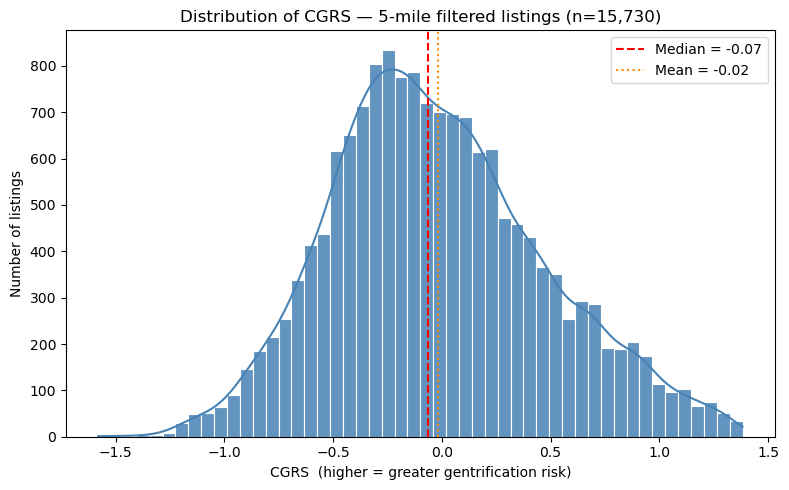
\includegraphics[width=0.75\textwidth]{figures/eda_cgrs_histogram.png}
\caption{Frequency distribution of the Composite Gentrification Risk Score across listings within five miles of a Metro station ($n=15{,}730$ in the visualized, percentile-capped subset).}
\label{fig:cgrs_hist}
\end{figure}

The Composite Gentrification Risk Score had a mean of approximately 0.00 and a standard deviation of 0.559 in the filtered sample, consistent with its z-score construction, which centers the distribution at zero (Figure~\ref{fig:cgrs_hist}). The median CGRS was $-0.061$, indicating that a majority of listings fall slightly below the average gentrification-risk level. The 25th and 75th percentiles were $-0.361$ and $0.306$, respectively, and the distribution showed a pronounced right skew with a maximum value of $25.098$, reflecting a small number of high-pressure listings with extreme scores across multiple components.

\begin{figure}[ht]
\centering
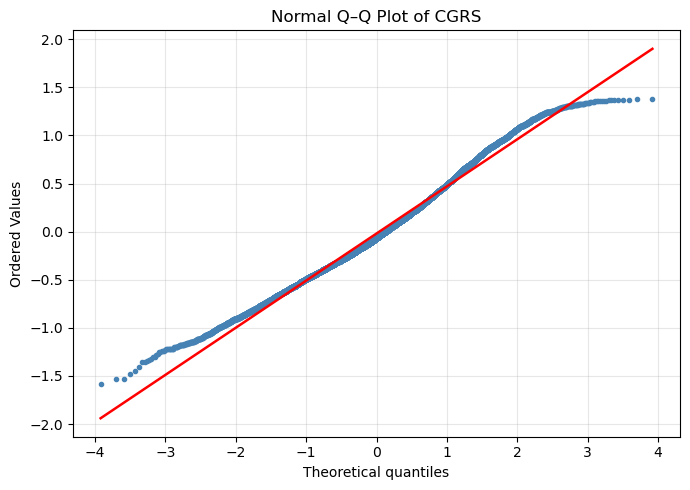
\includegraphics[width=0.62\textwidth]{figures/eda_cgrs_qqplot.png}
\caption{Normal Q--Q plot of the Composite Gentrification Risk Score, showing departure from the theoretical normal line in the upper tail.}
\label{fig:qq}
\end{figure}

A Shapiro-Wilk normality test on a random subsample of 5,000 listings returned $W = 0.987$, $p < 0.001$, confirming that the CGRS distribution is statistically non-normal. The Q--Q plot in Figure~\ref{fig:qq} corroborates this finding, with marked departure from the theoretical normal line at the upper tail. This non-normality motivated our choice of non-parametric tests in subsequent analyses and supported the use of tree-based models, which do not assume normally distributed residuals, over purely linear approaches.

\subsubsection{Transit Proximity and Gentrification Risk: TOD vs.\ Non-TOD}

\begin{figure}[ht]
\centering
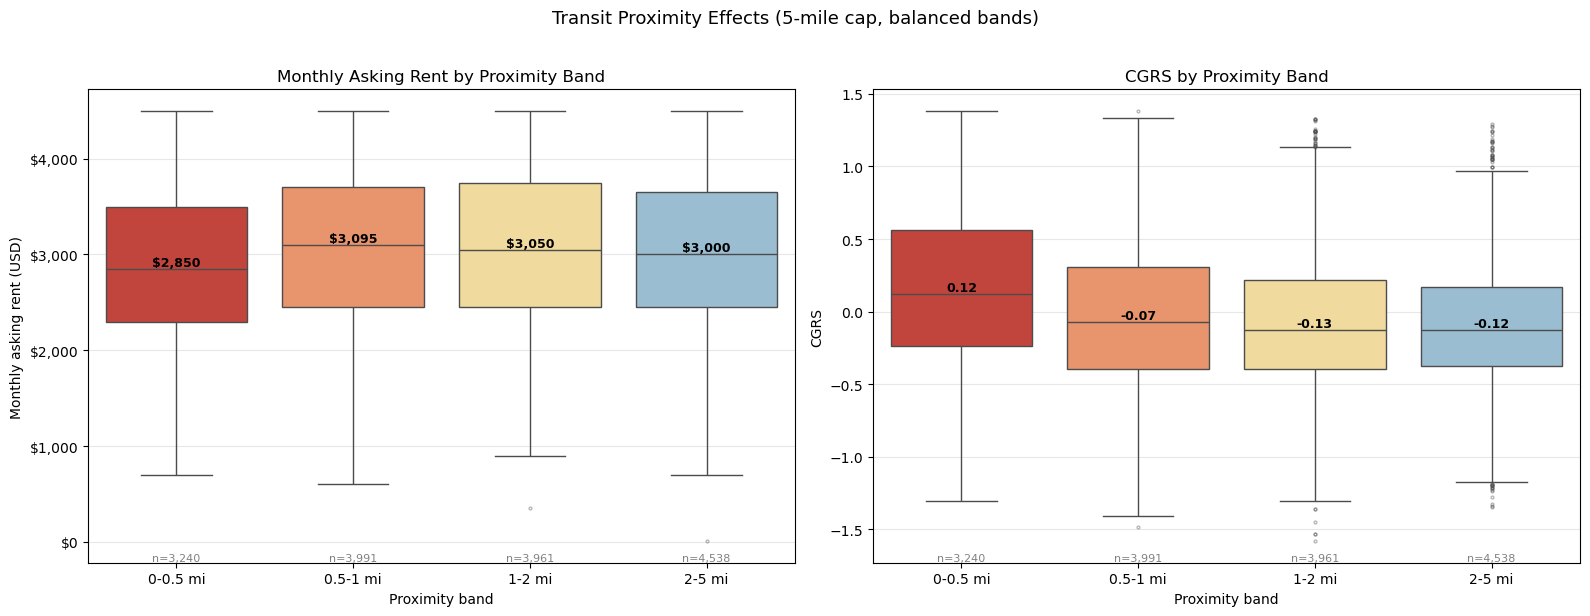
\includegraphics[width=0.95\textwidth]{figures/eda_band_boxplots.png}
\caption{Rent (left) and CGRS (right) by proximity band, with sample sizes annotated for each band (5-mile cap, balanced bands).}
\label{fig:band_box}
\end{figure}

To test whether listings near Metro stations exhibit higher gentrification risk than listings farther away, we compared CGRS distributions for listings inside and outside the 0.5-mile TOD buffer using a one-sided Mann-Whitney $U$ test. Listings within the TOD buffer ($n=3{,}240$) had a median CGRS of $0.125$, compared with a median of $-0.112$ for listings outside the buffer ($n=12{,}490$). The test returned $U = 25{,}290{,}586$, $p<0.001$, confirming that the difference is statistically significant at the 0.05 level (Figure~\ref{fig:band_box}).

This result supports the TOD-gentrification hypothesis drawn from \citet{kahn2007gentrification}: listings within walking distance of a Metro station are systematically associated with higher composite gentrification risk than listings farther away. A Kruskal-Wallis test across all Metro lines returned $H = 1{,}326.48$, $p<0.001$, indicating that CGRS distributions differ significantly across corridors, and that line identity carries meaningful information about a corridor's gentrification context.

\subsubsection{Distance-Decay of Gentrification Risk}

\begin{figure}[ht]
\centering
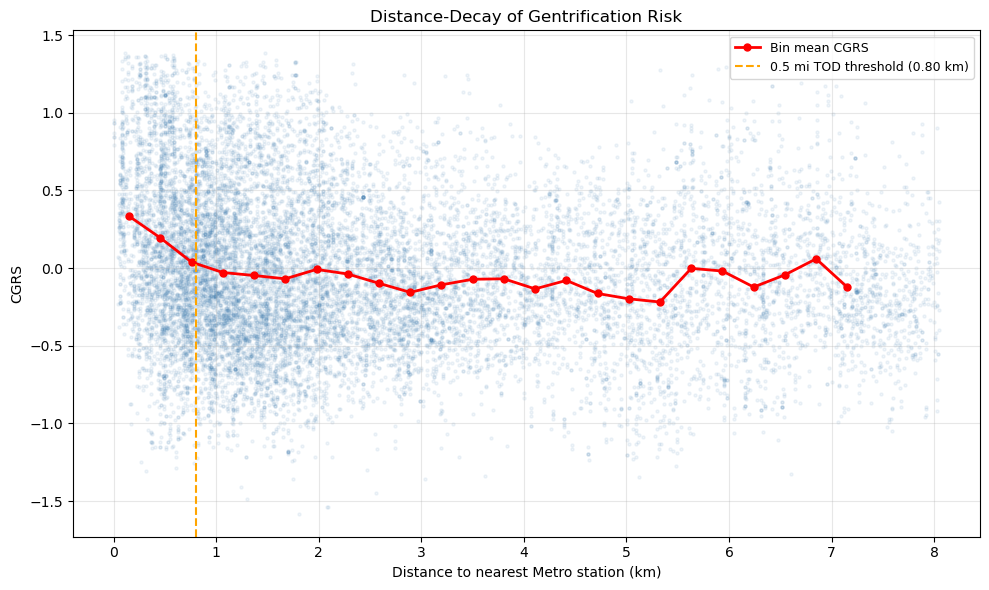
\includegraphics[width=0.78\textwidth]{figures/eda_distance_decay.png}
\caption{Distance-decay of mean CGRS, binned by distance to the nearest Metro station (25 equal-width bins from 0 to the 97th percentile of distance), with the 0.5-mile TOD threshold marked.}
\label{fig:decay}
\end{figure}

Figure~\ref{fig:decay} bins listings by distance to the nearest station and plots mean CGRS within each bin. The resulting curve declines roughly monotonically with distance, consistent with the theoretical prediction in \citet{nilsson2018transit} that gentrification risk falls off smoothly as distance from transit increases, and reinforcing the TOD-buffer finding above.

\subsubsection{Long-Term Gentrification Score (LTGS) by Line}

\begin{figure}[ht]
\centering
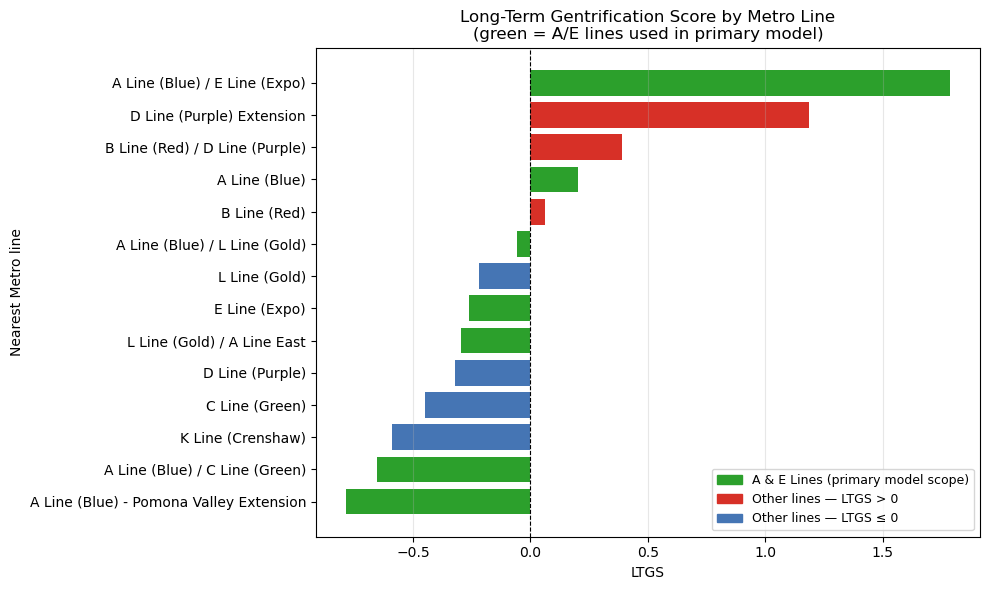
\includegraphics[width=0.78\textwidth]{figures/eda_ltgs_ranking.png}
\caption{Long-Term Gentrification Score (LTGS) by Metro corridor. The A and E Line corridors rank highest among existing lines, with a combined LTGS of approximately 1.8.}
\label{fig:ltgs}
\end{figure}

To evaluate whether restricting model training to the A and E Lines biases the analysis toward atypical corridors, we constructed a Long-Term Gentrification Score (LTGS) that aggregates three line-level signals into a single ranking:
\[
\text{LTGS} = \frac{1}{3}\Big[ z(\text{median CGRS}) + z(\text{mean SRA}) + z(\text{mean EDC}) \Big].
\]
Unlike the listing-level CGRS, LTGS characterizes an entire corridor rather than an individual unit. As shown in Figure~\ref{fig:ltgs}, the A and E Line corridors rank at or near the top of all existing Metro lines (combined LTGS $\approx 1.8$), confirming that they are not low-pressure outliers; if anything, they represent corridors that have already experienced substantial long-run gentrification pressure -- which is precisely the kind of corridor the Westwood/UCLA segment of the D Line is expected to resemble.

\subsection{Machine Learning Design and Model Performance}

\begin{table}[ht]
\centering
\caption{Five-fold cross-validated model performance, A/E-line training subset ($n=4{,}496$).}
\label{tab:ae_perf}
\begin{tabular}{lccc}
\toprule
\rowcolor{tableheader}
\textbf{Model} & \textbf{CV-RMSE (mean $\pm$ s.d.)} & \textbf{CV-MAE} & \textbf{CV-$R^2$} \\
\midrule
OLS / Ridge       & $0.376 \pm 0.014$ & 0.286   & $0.453$ \\
Random Forest     & $0.201 \pm 0.006$ & 0.144    & $0.844$ \\
XGBoost (best)    & $\mathbf{0.173 \pm 0.005}$ & 0.121    & $\mathbf{0.885}$ \\
\bottomrule
\end{tabular}
\end{table}

\begin{table}[ht]
\centering
\caption{Five-fold cross-validated model performance, all-lines robustness subset.}
\label{tab:all_perf}
\begin{tabular}{lccc}
\toprule
\rowcolor{tableheader}
\textbf{Model} & \textbf{CV-RMSE (mean $\pm$ s.d.)} & \textbf{CV-MAE} & \textbf{CV-$R^2$} \\
\midrule
OLS / Ridge       & $0.453 \pm 0.088$ & 0.321 & $0.343$ \\
Random Forest     & $0.253 \pm 0.127$ & 0.142 & $0.790$ \\
XGBoost           & $0.268 \pm 0.131$ & 0.125 & $0.757$ \\
\bottomrule
\end{tabular}
\end{table}

\begin{figure}[ht]
\centering
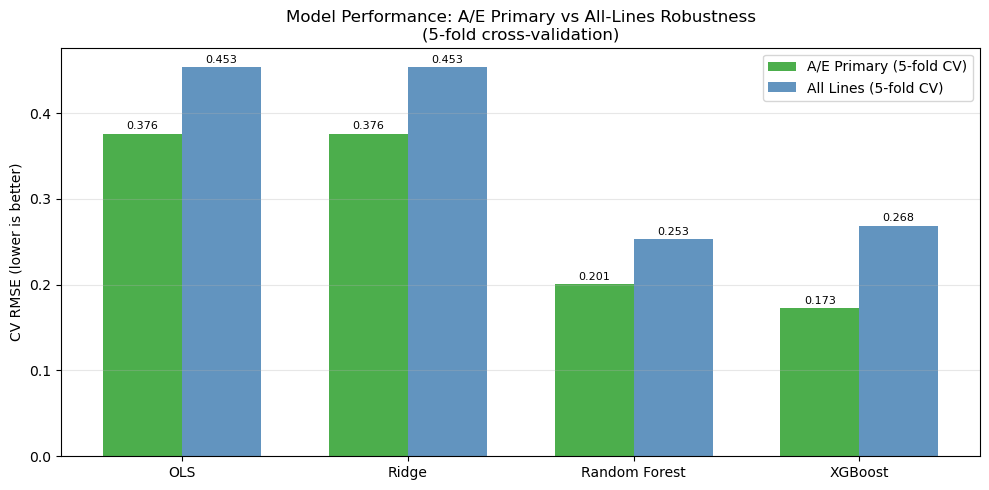
\includegraphics[width=0.85\textwidth]{figures/robustness_ae_vs_all.png}
\caption{Cross-validated RMSE for the A/E-line (primary) and all-lines (robustness) training subsets, by model. The A/E subset achieves both lower error and lower across-fold variance for every nonlinear model.}
\label{fig:robustness}
\end{figure}

Tables~\ref{tab:ae_perf}--\ref{tab:all_perf} and Figure~\ref{fig:robustness} compare model performance on the A/E-line training subset ($n=4{,}496$, mean CGRS $=0.054$, s.d.\ $=0.509$) against an identical 5-fold cross-validation run on all Metro lines. XGBoost is the strongest model on the A/E subset (CV-RMSE $=0.173 \pm 0.005$, CV-$R^2 = 0.885$), improving on Random Forest (CV-RMSE $=0.201 \pm 0.006$) and substantially outperforming the linear OLS/Ridge baseline (CV-RMSE $=0.376 \pm 0.014$, CV-$R^2=0.453$), which struggles with CGRS's right skew and the nonlinear, threshold-like behavior of the TOD effect.

Critically, every nonlinear model performs \emph{better and more stably} on the A/E subset than on the all-lines subset: XGBoost's CV-RMSE rises from $0.173$ to $0.268$ (a roughly 36\% degradation) and its across-fold standard deviation balloons from $0.005$ to $0.131$ when trained on all lines. This is strong empirical support for the A/E restriction described in Section~2.4: corridors such as the C/K Lines (confounded by LAX proximity) and the Pomona extension of the A Line (confounded by outer-suburban demographics that bear little resemblance to Westwood) inject heterogeneity that a single model cannot resolve, inflating both error and variance. The A/E model is therefore the theoretically -- and empirically -- preferred basis for the Olympics forecast, because it is trained on corridors most similar to the context the D Line Westwood extension will create.

\begin{figure}[ht]
\centering
\begin{subfigure}[b]{0.48\textwidth}
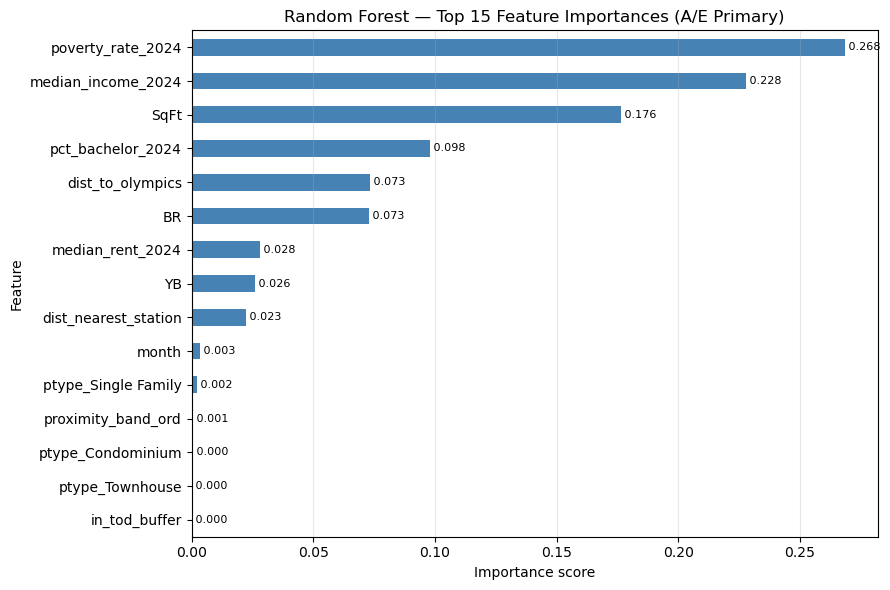
\includegraphics[width=\textwidth]{figures/ml_rf_importance.png}
\caption{Random Forest}
\end{subfigure}
\hfill
\begin{subfigure}[b]{0.48\textwidth}
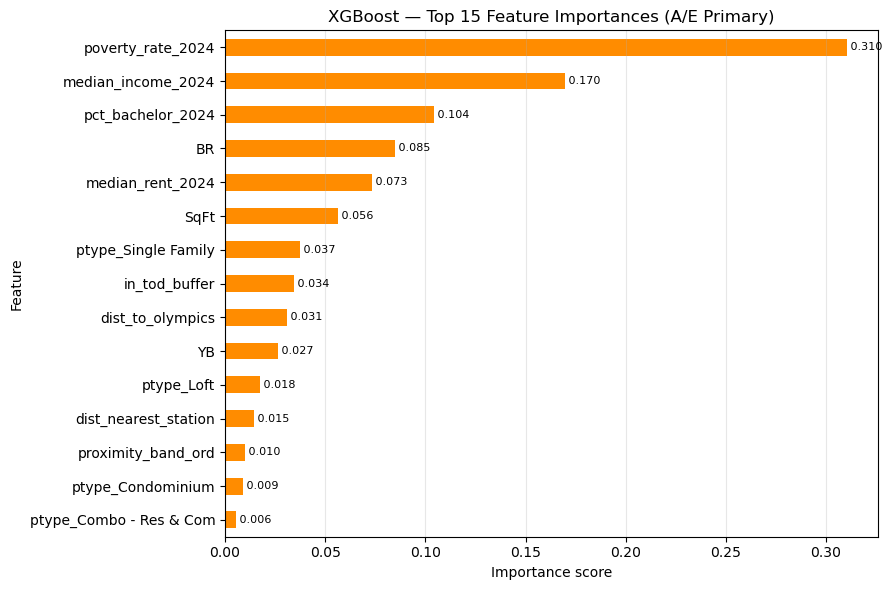
\includegraphics[width=\textwidth]{figures/ml_xgb_importance.png}
\caption{XGBoost}
\end{subfigure}
\caption{Top 15 feature importances (mean decrease in impurity / average gain) for the A/E Random Forest and XGBoost models. In both models, ZIP-level socioeconomic variables -- poverty rate, median income, and educational attainment -- dominate, with transit-distance variables (\texttt{dist\_to\_olympics}) ranking lower but still present among the top predictors.}
\label{fig:importance}
\end{figure}

Figure~\ref{fig:importance} shows the top 15 feature importances for the Random Forest and XGBoost A/E models. In the Random Forest, \texttt{poverty\_rate\_2024} (0.268), \texttt{median\_income\_2024} (0.228), and \texttt{SqFt} (0.176) are the leading predictors, followed by \texttt{pct\_bachelor\_2024} (0.098) and \texttt{dist\_to\_olympics} together with \texttt{BR} (0.073 each). When talking about XGBoost the ranking is similar: \texttt{poverty\_rate\_2024} (0.310), \texttt{median\_income\_2024} (0.170), \texttt{pct\_bachelor\_2024} (0.104), \texttt{BR} (0.085), and finally for \texttt{median\_rent\_2024} (0.073). We emphasize that these importances are a \emph{byproduct} of how the tree-based models partition the feature space -- not a feature-selection procedure -- and should be read descriptively: they indicate which variables the models leaned on most heavily to reduce prediction error, not which variables ``cause'' gentrification. The dominance of ZIP-level socioeconomic variables over unit-level and even transit-distance variables is itself informative, however: it suggests that neighborhood economic context, more than any single listing's characteristics or its proximity to a station, drives most of the variation in CGRS that these models can explain.

\begin{figure}[ht]
\centering
\begin{subfigure}[b]{0.48\textwidth}
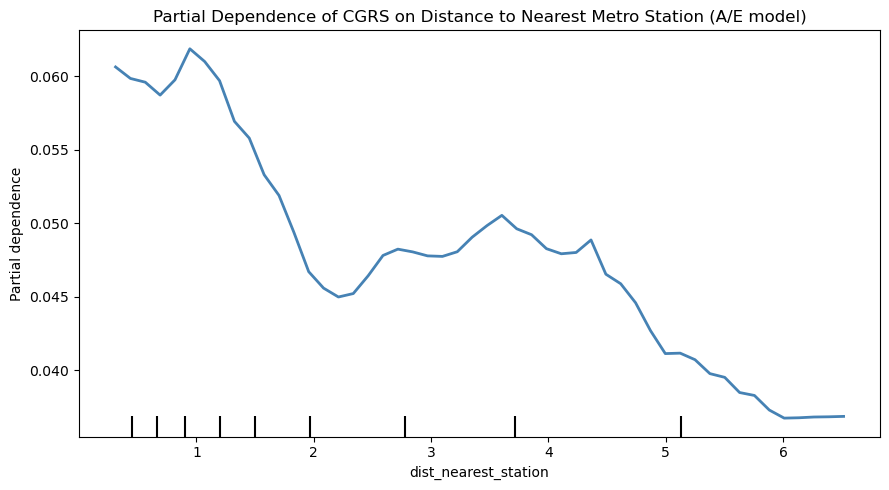
\includegraphics[width=\textwidth]{figures/ml_pdp_dist_nearest.png}
\caption{\texttt{dist\_nearest\_station}}
\end{subfigure}
\hfill
\begin{subfigure}[b]{0.48\textwidth}
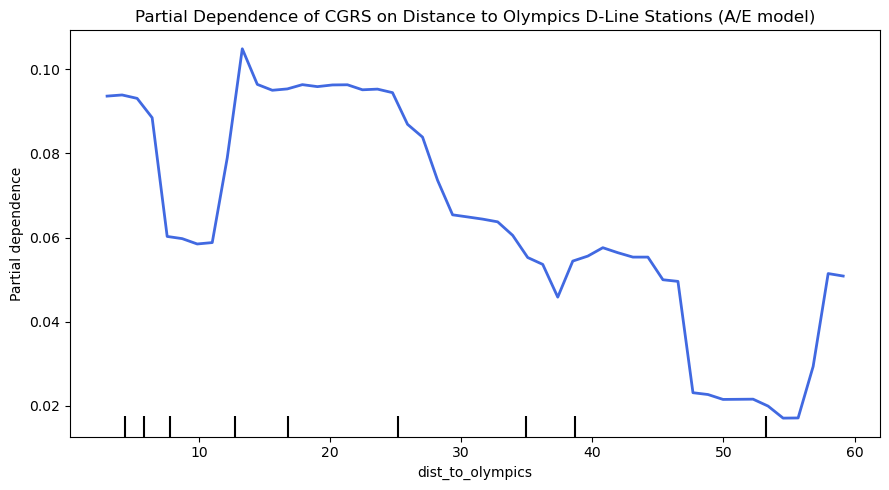
\includegraphics[width=\textwidth]{figures/ml_pdp_dist_olympics.png}
\caption{\texttt{dist\_to\_olympics}}
\end{subfigure}
\caption{Partial dependence plots for the two transit-distance predictors in the A/E Random Forest model, showing the marginal relationship between each distance variable and predicted CGRS, holding all other features at their observed distribution.}
\label{fig:pdp}
\end{figure}

The partial dependence plots in Figure~\ref{fig:pdp} isolate the marginal relationship between each transit-distance variable and predicted CGRS. Both curves show the model's learned, non-monotonic response to proximity -- predicted CGRS is highest in the immediate station vicinity and declines (with some local variation) as distance increases, mirroring the empirical distance-decay pattern in Figure~\ref{fig:decay} and the TOD-buffer effect documented in Section~3.2.2.

\subsection{Olympics D Line Extension Forecast}

\subsubsection{Counterfactual Design}

The forecast simulates what CGRS would look like near the D Line Extension stations after they open. This is a counterfactual exercise: we ask \emph{``what if these stations existed, and listings near them were as close to a station and as transit-accessible as listings already inside the TOD buffer?''} Specifically, for every listing within five kilometers of the four planned Olympic-corridor stations, we construct a counterfactual feature vector by (1) setting \texttt{dist\_to\_olympics} $= 0.3$ km, representative of walking distance to a station and within the TOD buffer; (2) setting \texttt{in\_tod\_buffer} $=1$, reflecting that the listing would be transit-accessible at opening; and (3) holding all other features -- demographics, rent, and unit characteristics -- constant. We then generate predictions under both the baseline (current distances) and the post-opening (counterfactual distances) scenarios using the trained A/E Random Forest model. The difference between the two predictions, for each listing, is the estimated uplift attributable specifically to the arrival of transit.

\subsubsection{Interpreting the Forecast}

\begin{figure}[ht]
\centering
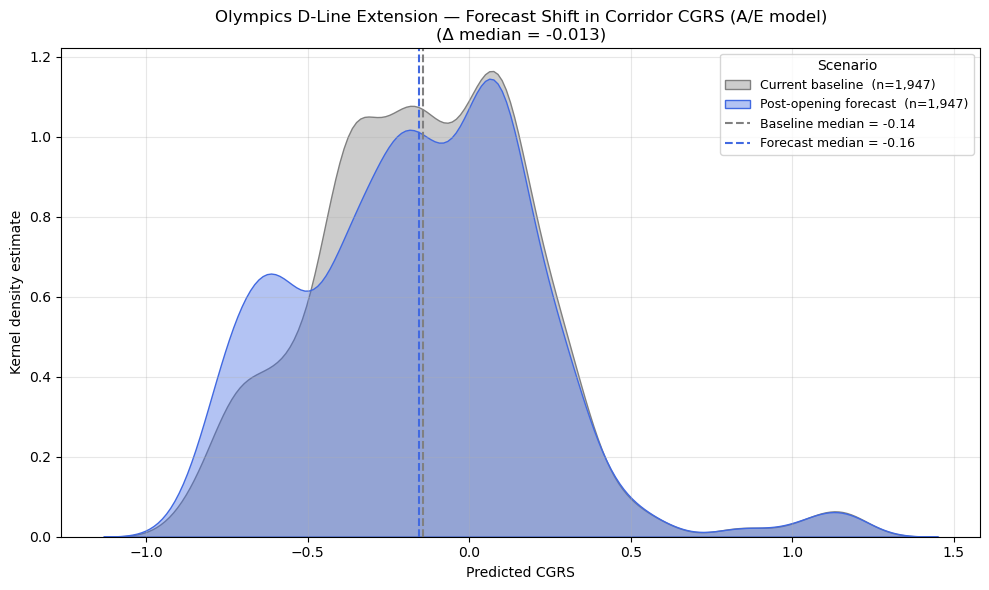
\includegraphics[width=0.78\textwidth]{figures/forecast_cgrs_kde.png}
\caption{Kernel density estimate of predicted CGRS in the Olympic Corridor, baseline vs.\ post-opening counterfactual (A/E model). Baseline median $\approx -0.14$; forecast median $\approx -0.16$; median shift $\Delta \approx -0.013$.}
\label{fig:kde}
\end{figure}

\begin{figure}[ht]
\centering
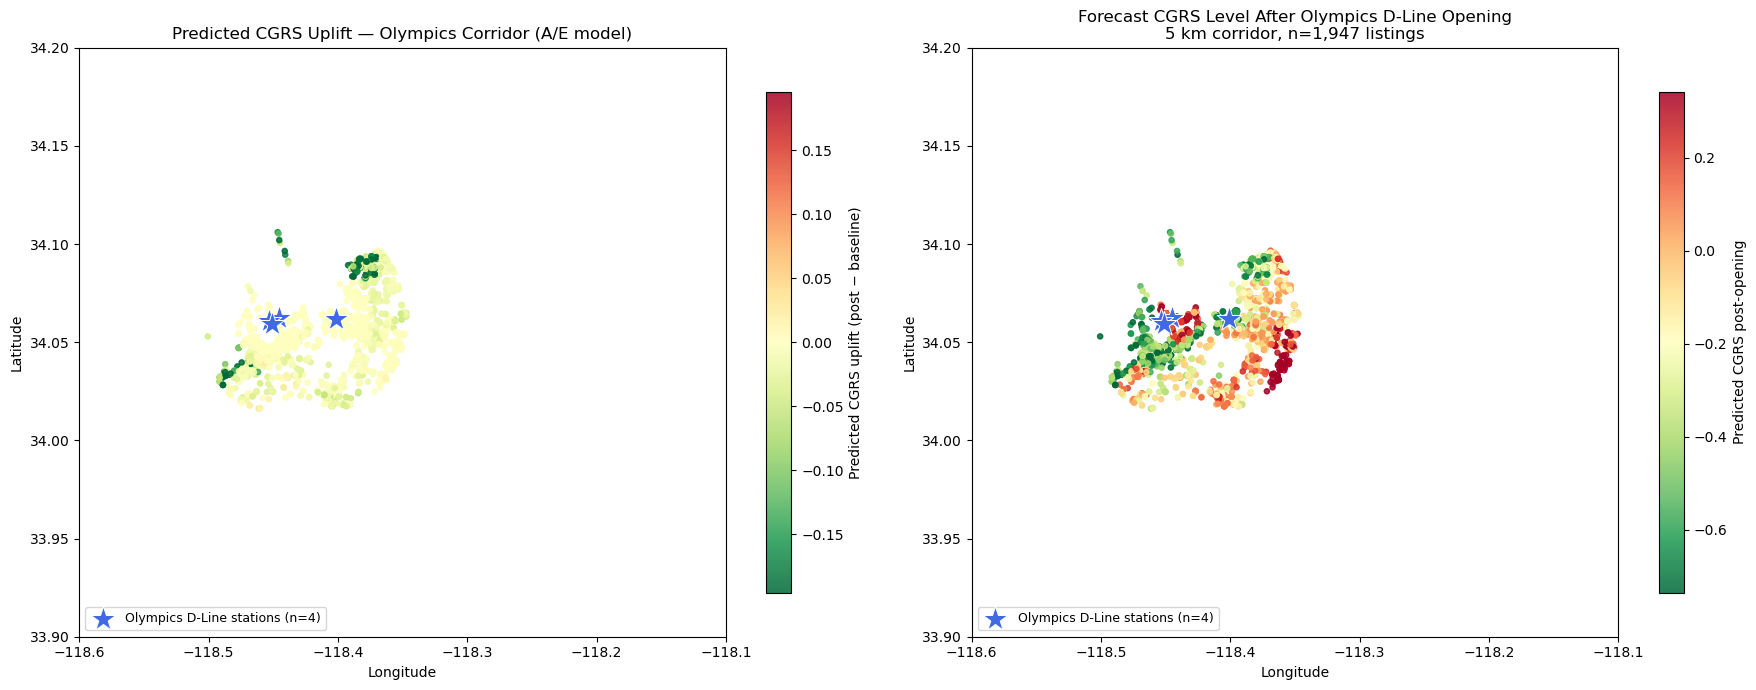
\includegraphics[width=0.95\textwidth]{figures/forecast_uplift_map.png}
\caption{Spatial maps of the Olympic Corridor: predicted CGRS uplift attributable to the D Line Extension (left) and predicted post-opening CGRS level (right).}
\label{fig:uplift_map}
\end{figure}

The uplift map (Figure~\ref{fig:uplift_map}, left) shows the marginal CGRS increase attributable specifically to transit arrival, while the post-opening map (right) shows the combined level of risk -- baseline plus uplift. Both views are necessary, because a listing can show high uplift but low absolute CGRS (transit arriving in a currently low-risk area -- a watchlist candidate for future gentrification), or low uplift but high absolute CGRS (an area already at high risk, where transit adds only marginally to an already-pressured market).

The KDE shift plot (Figure~\ref{fig:kde}) shows the full predicted-CGRS distribution before and after opening for the 1,947 corridor listings in the forecast set. The mean uplift is $-0.027$ and the median uplift is $-0.0023$, with only 21.5\% of listings showing a positive (gentrification-increasing) shift; the median CGRS level itself shifts from approximately $-0.14$ to $-0.16$ ($\Delta \text{median} \approx -0.013$). Disaggregating by proximity band, the median uplift is $-0.0023$ for 0--0.5 mi listings ($n=404$), $-0.0006$ for 0.5--1 mi ($n=968$), $-0.0114$ for 1--2 mi ($n=566$), and $-0.1229$ for the small 2--5 mi group ($n=9$). In every band, the median shift is at or near zero, and the overall pattern is consistent with the ``ceiling effect'' hypothesis described in \citet{nilsson2018transit}: an already-high-CGRS corridor has limited additional room for transit arrival, by itself, to push the index meaningfully higher.

% =====================================================================
\section{Discussion}
% =====================================================================

This study attempts to measure the possibility of gentrification in the Olympic Corridor prior to the opening of the LA Metro Rail D Line Extension. The forecast works by running each listing through the trained model twice -- once with its real, current distances, and once with distances artificially set to simulate the new D Line stations being open. The difference between the two predictions is the uplift: the added gentrification pressure attributable specifically to the arrival of transit. In the Westwood/UCLA corridor, the predicted uplift is near zero -- small enough that we can say the new stations are unlikely to have a meaningful, transit-attributable effect on gentrification risk in the immediate area. The baseline CGRS in the corridor is already high before the stations even open, which suggests that existing market forces have already produced much of the change this study set out to measure. The more plausible site of real displacement risk is in adjacent, still-affordable neighborhoods such as Koreatown, Palms, and Mar Vista, where improved regional accessibility from the D Line Extension could attract higher-income residents without the same income-and-rent ceiling dampening the effect.

\subsection{The A/E Restriction as a Design Decision}

The most consequential design decision in this project was which Metro corridors to train the prediction model on. We considered two approaches: training on listings near any Metro line in LA County, or restricting training to listings whose nearest station is on the A or E Line.

The first option maximizes the available training data -- roughly 21,000 listings -- but pools together corridors with fundamentally different characteristics. Lines such as the C or K, which run adjacent to LAX, carry rents elevated by proximity to a major international airport -- a qualitatively different mechanism that would confound the model. The Pomona extension of the A Line runs through outer-suburban Azusa and Pomona, whose demographics and housing markets bear little resemblance to Westwood or Beverly Hills, and the J Line -- a Bus Rapid Transit corridor -- does not fit cleanly within the rail-based TOD literature this study draws on.

The second option, which we adopted, restricts training to listings whose nearest station sits on the A or E Line. These corridors share key characteristics with the planned D Line Westwood extension: an east-west geographic alignment (the A Line through South LA, the E Line through Culver City and Santa Monica) and comparable urban density. The socioeconomic variation across the A and E corridors also spans a range of income levels relevant to what the D Line extension is likely to encounter. The tradeoff is a smaller training set (roughly 4,500--7,000 listings, depending on the distance filter); however, as Section~3.3 demonstrates empirically, the gain in transferability to the D Line corridor -- reflected in both lower error \emph{and} lower across-fold variance -- outweighs the cost of the smaller sample, and the restriction was adopted because it more narrowly targets the research question.

\subsection{Implications for the Westwood/UCLA Corridor}

Our findings suggest that concerns about transit-induced gentrification in the immediate Westwood/UCLA segment of the D Line Extension may not carry the same weight as similar concerns raised about other Metro rail openings. While the corridor already exhibits high baseline gentrification risk, the model indicates that the opening of new stations is unlikely to substantially raise that risk beyond its existing level. This distinction matters for planners and policymakers: it suggests that, in already high-cost neighborhoods, transit investment alone is not necessarily the primary driver of additional displacement pressure.

\subsection{Implications for Surrounding Communities and Housing Policy}

At the same time, our results indicate that displacement pressure may emerge in nearby communities where housing costs remain comparatively lower and where improved regional accessibility could draw higher-income residents. Anti-displacement interventions should therefore not be limited to the immediate vicinity of new stations; local governments should consider proactive protections in adjacent communities likely to experience secondary effects of transit expansion.

These findings also carry broader housing-policy implications. Transit-oriented development is often promoted as a strategy for reducing automobile dependence and improving access to employment centers, yet its benefits can be unevenly distributed when housing supply and affordability are not addressed at the same time. Expanding affordable-housing requirements near transit corridors, preserving existing rent-stabilized units, and strengthening tenant protections may help ensure that the benefits of transit investment are shared across income groups. Monitoring the behavior of large corporate landlords and institutional property owners in neighborhoods experiencing rising transit accessibility may also help identify emerging displacement pressures before they become entrenched.

\subsection{Value of Predictive, Pre-Opening Analysis}

More broadly, this study illustrates the value of predictive modeling for identifying neighborhoods that may be vulnerable to future gentrification pressure. By estimating likely changes \emph{before} infrastructure projects are completed, planners can target mitigation efforts proactively, rather than responding only after displacement has already occurred.

\subsection{Limitations}

Several limitations attenuate these results. First, the rental-price data span a relatively narrow one-year window. Because this period roughly matches typical lease lengths, we could not track changes in asking price for the same listings over time, making the data functionally cross-sectional; true mediation effects of the Metro opening on gentrification cannot be examined with the current dataset. Future work could strengthen this design by adding controls for change in rental prices over time, population density, and markers for jurisdictions with independent rent-control regimes (such as Santa Monica and West Hollywood).

Second, existing Metro lines already run through some of the most expensive parts of LA, and this study cannot determine whether the lines contributed to that expense or were sited in already-popular, dense areas. This raises a substantial possibility of a ceiling effect: in corridors such as the Olympic Corridor, where many hallmarks of gentrification are already present, predicting \emph{further} gentrification in an already-saturated market can yield diminishing, hard-to-detect returns -- which is consistent with the near-zero uplift we estimate.

Finally, this study relies on a modeled gentrification-risk score rather than on observed measures of displacement or neighborhood change. Predicted increases in risk should therefore be read as indicators of potential vulnerability, not as direct evidence that gentrification or displacement will occur.

% =====================================================================
\section{Conclusion}
% =====================================================================

This study examined the potential impact of the Los Angeles Metro D Line Extension on gentrification risk in the Olympic Corridor, using a predictive-modeling approach that simulates the accessibility changes associated with new transit stations. The results suggest that the Olympic Corridor is unlikely to experience substantial \emph{additional} gentrification pressure as a direct result of the D Line Extension, largely because the area already exhibits high baseline levels of gentrification risk. Instead, transit-related displacement pressure may be more likely to emerge in nearby, relatively affordable neighborhoods that stand to gain improved regional accessibility. While the study is limited by its cross-sectional design and the data available, it demonstrates the value of predictive models for flagging areas of concern before major infrastructure projects are completed -- giving policymakers and planners a window in which to design interventions that balance the benefits of transit investment with housing stability and affordability.

% =====================================================================
\bibliographystyle{plainnat}
\bibliography{references}

\end{document}
